
%(BEGIN_QUESTION)
% Copyright 2005, Tony R. Kuphaldt, released under the Creative Commons Attribution License (v 1.0)
% This means you may do almost anything with this work of mine, so long as you give me proper credit

Suppose you needed to choose a potentiometer value ($R$) to make a voltage divider circuit, given a known fixed resistor value, the source voltage value, and the desired range of adjustment:

$$\includegraphics[width=15.5cm]{i03132x01.eps}$$

Solve for $R$, and show the equation you set up in order to do it.  Also, determine the respective potentiometer wiper positions at 0 volts and at 17 volts.


\vfil 

\underbar{file i03132}
\eject
%(END_QUESTION)





%(BEGIN_ANSWER)

This is a graded question -- no answers or hints given!

%(END_ANSWER)





%(BEGIN_NOTES)

$$17 = 24 \left(R \over {50000 + R} \right)$$

$$17 (50000 + R) = 24R$$

$$850000 + 17R = 24R$$

$$850000 = 7R$$

$$R = 121.43 \hbox{ k} \Omega $$

\vskip 10pt

The potentiometer wiper will be fully {\it up} 1t 0 volts and fully {\it down} at 17 volts.

%INDEX% Mathematics review: manipulating literal equations

%(END_NOTES)


